\section{Compiling and Running \D}
\label{compilation}

When you have obtained \D from Daresbury Laboratory and unpacked it,
your next task will be to compile it.

CMake - \href{http://www.cmake.org/}{http://www.cmake.org/}\index{WWW} - is
an open-source, cross-platform family of tools designed to build, test
and package software.  CMake is used to control the software compilation
process using simple platform and compiler independent configuration files,
and generate native makefiles and workspaces that can be used in a
compiler environment of your choice.  The suite of CMake tools was
created by Kitware in response to the need for a powerful, cross-platform
build environment for open-source projects such as ITK, VTK, KDE, etc...

In order to build a \D executable with cmake there are two stages -
{\bf Stage~1}: generating the build files (e.g. makefiles); and
{\bf Stage~2}: building the code (e.g. make).

For the examples within this section we assume that \D has been
downloaded, the archived contents extracted and we are stepped in the
the main folder (root).  All commands and discussions that follow are
relative to this root folder of \D.

Full instructions can be also found online at \url{https://ccp5.gitlab.io/dlpoly-setup/}

\begin{itemize}
\item {\bf Stage~1}: Configure and generate the build files. \\

One can pass different options to the build system to generate
the build files.  It is important to determine these before one
choses the ones they consider relevant for their purposes.
Finding out all available options for \D can be done in the
following ways:

\begin{enumerate}[label=\textbf{\alph*)}]%,start=0]
\item by using {\sl cmake}:
\begin{lstlisting}
[10:38:02 alin@abaddon:~/playground/dl-poly]: mkdir myBuild
[10:38:11 alin@abaddon:~/playground/dl-poly]: cd myBuild/
[10:38:13 alin@abaddon:~/playground/dl-poly/myBuild]: cmake .. -L
....
-- Cache values
BUILDER:STRING=
BUILD_SHARED_LIBS:BOOL=OFF
BUILD_TESTING:BOOL=OFF
CMAKE_BUILD_TYPE:STRING=
CMAKE_INSTALL_PREFIX:PATH=/usr/local
DOCS:BOOL=OFF
HOST:STRING=abaddon.dl.ac.uk
MPI_NPROCS:STRING=8
WITH_COVERAGE:BOOL=OFF
WITH_EXTRATIME:BOOL=OFF
WITH_FORCHECK:BOOL=OFF
WITH_KIM:BOOL=OFF
WITH_MPI:BOOL=ON
WITH_NETCDF:BOOL=OFF
WITH_OPENMP:BOOL=OFF
WITH_PHI:BOOL=OFF
WITH_PLUMED:BOOL=OFF
\end{lstlisting}

Do notice that some of the options are already filled in...
{\em cmake} already tried its best to find some of the
available information about your system and picked the some
defaults, a.g. {\bf WITH\_MPI:BOOL=ON}.

\item by reading the \D option file: \\
All available options and their description are stored in
{\sc cmake/DLPOLYBuildOptions.cmake}.
\begin{lstlisting}
[10:46:01 alin@abaddon:~/playground/dl-poly]: cat cmake/DLPOLYBuildOptions.cmake
option(WITH_MPI "build a MPI version" ON)
option(WITH_OPENMP "build an OpenMP version" OFF)
option(WITH_PHI "build an executable for Xeon Phi version" OFF)
option(WITH_NETCDF "build using netcdf support version" OFF)
option(WITH_EXTRATIME "activate extra timing information" OFF)
option(WITH_KIM "Build with KIM support" OFF)
option(WITH_PLUMED "Build with PLUMED support" OFF)
option(BUILD_TESTING "Build with Testing support" OFF)
option(WITH_COVERAGE "Build with instrumentation for code coverage" OFF)
option(WITH_FORCHECK "Build with forcheck for code" OFF)
option(DOCS "Doxygen Documentation" OFF)
option(BUILD_SHARED_LIBS "Build with shared libraries" OFF)

set(MPI_NPROCS 8 CACHE STRING "number of MPI processes to be used for code coverage and tests")
cmake_host_system_information(RESULT AH QUERY FQDN)
set(HOST "${AH}" CACHE STRING "name of the hostname we build on.")
set(BUILDER "" CACHE STRING "name of the person who built the binary.")
\end{lstlisting}

\item by using {\sl ccmake}: \\
Press $<$c$>$ to configure and $<$e$>$ if errors appears.
A typical output is shown in Figure~\ref{ccmakefig}.
\begin{lstlisting}
[10:38:02 alin@abaddon:~/playground/dl-poly]: mkdir myBuild
[10:38:11 alin@abaddon:~/playground/dl-poly]: cd myBuild/
[10:38:13 alin@abaddon:~/playground/dl-poly/myBuild]: ccmake ..
\end{lstlisting}
\begin{figure}[htbp]
\begin{center}
\vskip 1ex
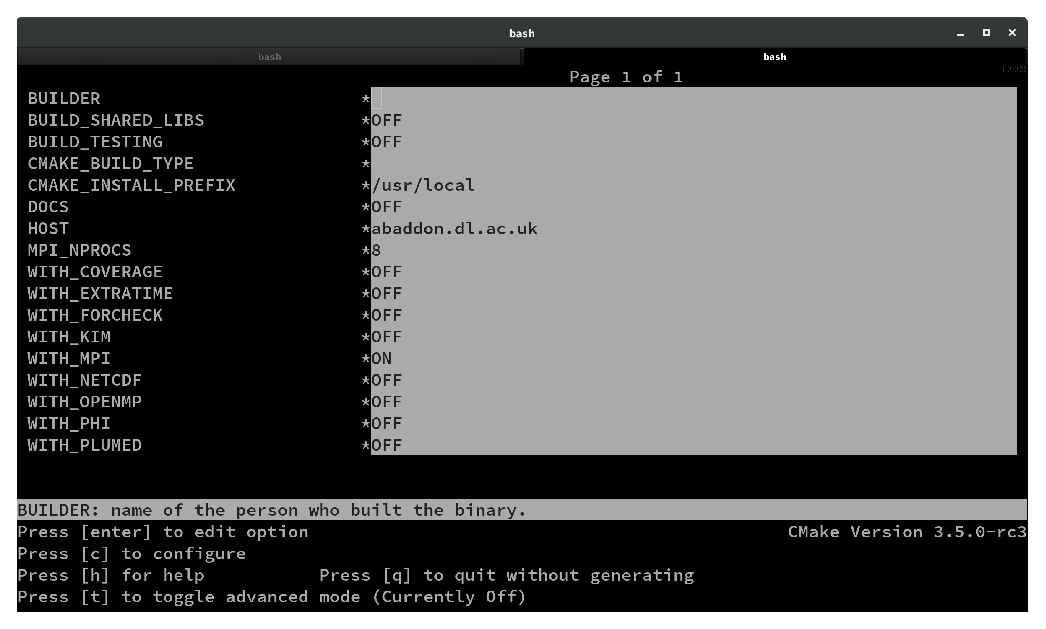
\includegraphics[height=9cm]{ccmake.eps}
\caption{Typical ccmake output for \D}
\label{ccmakefig}
%\vskip 1ex
\end{center}
\end{figure}

\item by using {\sl cmake-gui}: \\
A typical output is shown in Figure~\ref{ccmake-gui}.
\begin{lstlisting}
[10:38:02 alin@abaddon:~/playground/dl-poly]: mkdir myBuild
[10:38:11 alin@abaddon:~/playground/dl-poly]: cd myBuild/
[10:38:13 alin@abaddon:~/playground/dl-poly/myBuild]: cmake-gui ..
\end{lstlisting}
\begin{figure}[htbp]
\begin{center}
\vskip 1ex
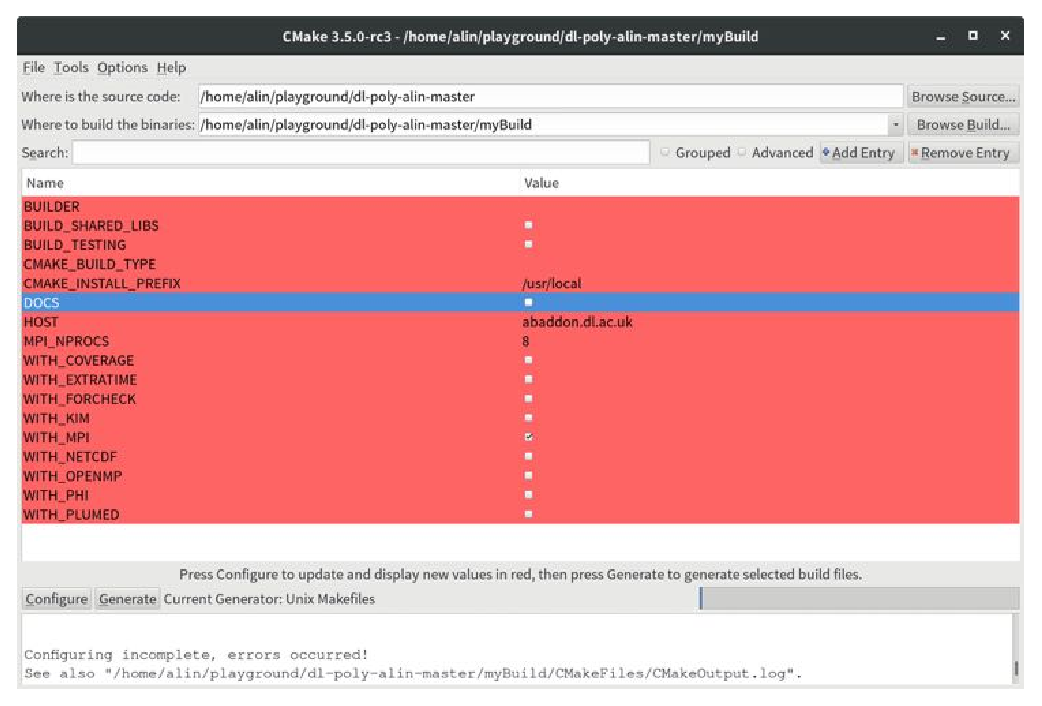
\includegraphics[height=11cm]{cmake-gui.eps}
\caption{Typical cmake-gui output for \D}
\label{ccmake-gui}
%\vskip 1ex
\end{center}
\end{figure}
\end{enumerate}

One may also choose to pass the command line options via {\bf -DOPTION=value}.
Explicit compiler specification can be achieved by setting the environment
variable {\bf FC} (e.g. using Intel ifort {\bf FC=ifort}).  Compiler flags
can be altered via {\bf FFLAGS}, (e.g. {\bf FFLAGS="-O3 -xHost"}).  Once one
is happy with the choices made then they are ready to move to Stage~2.

\item {\bf Stage~2}: Build the executable. \\

Building is as simple as typing {\sl make -jX}, where X is the number of
desired compilation threads to work in parallel.  Once the build process
is successful one can find the \D executable in the folder {\em bin}
(freshly generated if it did not exists before).  One can then copy or
link the executable to any accessible to them place on the system they wish.
\end{itemize}

{\bf Examples of different builds}.  Assuming that the OS environment
is set up properly so that access paths to the MPI library (and any
other needed libraries) and gfortran is the default FORTRAN90 compiler.
\begin{itemize}
\item {\bf Pure MPI}
\begin{lstlisting}
[alin@abaddon: ...dl-poly]: mkdir myBuild
[alin@abaddon: ...dl-poly]: cd myBuild/
[alin@abaddon: ...dl-poly/myBuild]: FFLAGS="-O3 -mtune=native" cmake ..
[alin@abaddon: ...dl-poly/myBuild]: make -j10
\end{lstlisting}

\item {\bf Serial}
\begin{lstlisting}
[alin@abaddon: ...dl-poly]: mkdir myBuild
[alin@abaddon: ...dl-poly]: cd myBuild/
[alin@abaddon: ...dl-poly/myBuild]: FFLAGS="-O3 -mtune=native" cmake .. -DWITH_MPI=OFF
[alin@abaddon: ...dl-poly/myBuild]: make -j10
\end{lstlisting}

\item {\bf Pure MPI+NETCDF}
\begin{lstlisting}
[alin@abaddon: ...dl-poly]: mkdir myBuild
[alin@abaddon: ...dl-poly]: cd myBuild/
[alin@abaddon: ...dl-poly/myBuild]: FFLAGS="-O3 -mtune=native" cmake .. -DWITH_NETCDF=ON
[alin@abaddon: ...dl-poly/myBuild]: make -j10
\end{lstlisting}

\item {\bf Pure MPI+KIM}
\begin{lstlisting}
[alin@abaddon: ...dl-poly]: mkdir myBuild
[alin@abaddon: ...dl-poly]: cd myBuild/
[alin@abaddon: ...dl-poly/myBuild]: FFLAGS="-O3 -mtune=native" cmake .. -DWITH_KIM=ON
[alin@abaddon: ...dl-poly/myBuild]: make -j10
\end{lstlisting}

\item {\bf Pure MPI+PLUMED}
\begin{lstlisting}
[alin@abaddon: ...dl-poly]: mkdir myBuild
[alin@abaddon: ...dl-poly]: cd myBuild/
[alin@abaddon: ...dl-poly/myBuild]: FFLAGS="-O3 -mtune=native" cmake .. -DWITH_PLUMED=ON
[alin@abaddon: ...dl-poly/myBuild]: make -j10
\end{lstlisting}

\item {\bf Pure MPI+Testing}
\begin{lstlisting}
[alin@abaddon: ...dl-poly]: mkdir myBuild
[alin@abaddon: ...dl-poly]: cd myBuild/
[alin@abaddon: ...dl-poly/myBuild]: FFLAGS="-O3 -mtune=native" cmake .. -DBUILD_TESTING=ON
[alin@abaddon: ...dl-poly/myBuild]: make -j10
\end{lstlisting}
To run the tests one can run {\sl make}~$test$ or {\sl ctest}.
For a complete list of tests available, run {\sl ctest -N}.
If specific test is desired to run then use {\sl ctest -R TESTNAME}.
\end{itemize}

For a list of complete options to build use {\sl make help}.  The list will be different
depending on the options used to configure.

\subsection{Note on the Interpolation Scheme}
\label{interpolation}

In \D two-body-like contributions (van der Waals\index{potential!van der Waals},
metal\index{potential!metal} and real space Ewald summation\index{Ewald!summation})
to energy and force are evaluated by interpolation of tables
constructed at the beginning of execution.  The \D interpolation
scheme is based on a 3-point linear interpolation in $r$.  {\bf Note}
that a 5-point linear interpolation in $r$ is ised in \D for
interpolation of the EAM (metal) forces from EAM table data (TABEAM).

The number of grid points ({\tt mxgrvdw}) required for interpolation in
$r$ to give good energy conservation in a simulation is:
\[ {\tt mxgrid} = {\tt Max}({\tt mxgrid}, 1004, {\tt Nint}(r_{\tt cut}/\delta r_{\tt max}) + 4)~~, \]
where $r_{\tt cut}$ is the main cutoff beyond which the contributions
from the short-range-like interactions are negligible, and $\delta r_{\tt max}~=~0.01$~\AA.
is the default grid bin for real space grids.

\subsection{Running}

To run the \D executable (DLPOLY.Z) you will initially require
at least three input data files, which you must provide in the
{\em execute} sub-directory, (or whichever sub-directory you will
execute the run).  The first of these is the CONTROL file
(Section~\ref{control-file}), which indicates to \D what kind of
simulation conditions you want to run, how much data you want to
gather and for how long you want the job to run.  The second file
you need is the CONFIG file (Section~\ref{config-file}).  This
contains the atom positions and, depending on how the file was
created (e.g. whether this is a configuration created from `scratch'
or the end point of a previous run), the velocities and forces also.
The third file required is the FIELD file (Section~\ref{field-file}),
which specifies the atomic properties (such as charge and mass),
molecular stoichiometry and intermolecular topology and interactions,
and finally intermolecular interactions and external fields.
Sometimes one or a few more extra files may also be required: MPOLES
(Section~\ref{mpoles-file}) - which contains the specification of
higher order charge distributions (multipolar momenta); TABLE
(Section~\ref{table-file}), TABEAM (Section~\ref{tabeam-file}),
TABBND, TABANG, TABDIH and TABINV Files (Section~\ref{intra-tables});
which contain potential and force arrays for particular type of
interaction that is not supplied with an explicit analytical for in
\D (usually because they are too complex, e.g. spline potentials,
, non-analytic functionals as in TEABEAM, etc.).  Other optional
files may also be required such as REFERENCE (Section~\ref{reference-file})
- similar to the CONFIG file it contains the "perfect" crystalline
structure of the system used as a reference to detect instantaneous
interstitial and vacancy defects during radiation damage events,
HISTORY (Section~\ref{history-file}) - used for replaying a previously
generated trajectory so that various observables could be recreated
(e.g. RDF, Z-density profiles, etc.).

Examples of input files are found in the {\em data} sub-directory,
which can be copied into the {\em execute} subdirectory using the {\sl
select} macro found in the {\em execute} sub-directory.

A successful run of \D will generate several data files, which
appear in the {\em execute} sub-directory.  The most obvious one
is the file OUTPUT (Section~\ref{output-file}), which provides an
effective summary of the job run: the input information; starting
configuration; instantaneous and rolling-averaged thermodynamic
data; minimisation information, final configurations;
radial distribution functions (RDFs); Z-density profiles
and job timing data.  The OUTPUT file is human readable.  Also
present will be the restart files REVIVE (Section~\ref{revive-file})
and REVCON (Section~\ref{revcon-file}).  REVIVE contains the
accumulated data for a number of thermodynamic quantities and
statistical accumulators (RDFs, fluctuations, etc.), and is
intended to be used as the input file for a following run.
It is {\em not} human readable.  The REVCON file contains the
{\em restart configuration}, i.e. the final positions, velocities
and forces of the atoms when the run ended and is human readable.
The STATIS file (Section~\ref{statis-file}) contains a catalogue
of instantaneous values of thermodynamic and other variables, in
a form suitable for temporal or statistical analysis.

There are quite a few other optional files, for which more detailed
description and formating can be found in the relevant
Section~\ref{output-files}.  It is, however, worth mentioning that
these are generated upon specific user instructions in CONTROL,
so their specific functional description and activation information
detail can be found in Section~\ref{control-file}.

\subsection{Parallel I/O}

Many users that have suffered loss of data in the OUTPUT, especially
running in parallel and when an error occurs on parallel architectures.
In such circumstances the OUTPUT may be empty or incomplete, despite
being clear that the actual simulation has progressed well beyond what
has been printed in OUTPUT.  Ultimately, this is due to OS's I/O
buffers not being flushed as a default by the particular OS when
certain kind of errors occurs, especially MPI related.  The safest way
to avoid loss of information in such circumstances is to write the
OUTPUT data to the default output channel ("the screen").  There is an
easy way to do this in \D, which is to use the {\bf l\_scr} keyword in
the CONTROL file.  The batch daemon will then place the output in the
standard output file, which can then be of use to the user, or
alternatively on many batch systems the output can be redirected into
another file, allowing an easier following of the job progress over
time.  This latter technique is also useful on interactive systems
where simply printing to the screen could lead to large amounts of
output.  However, such situations could be easily avoided by
redirecting the output using the "$>$" symbol, for instance:
"mpirun -n 4 DLPOLY.Z $>$ OUTPUT".

It is also worth noting that the use of large batch and buffer
numbers can speed up enormously the performance of the parallel I/O,
for example putting in CONTROL (see Section~\ref{control-file}):
\begin{lstlisting}
io read mpiio         128 10000000 1000000
io write mpiio        512 10000000 1000000
\end{lstlisting}
at large processor count jobs (over 1000).  However, this help comes
at a price as larger batches and buffers also requires more memory.
So at smaller processor counts the job will abort at the point of
trying to use some of the allocated arrays responsible for these.

More information about \D parallel I/O can be found in the following
references \cite{todorov-09a,todorov-08a,bush-10a}.

\subsection{Restarting}

The best approach to running \D is to define from the outset
precisely the simulation you wish to perform and create the input
files specific to this requirement.  The program will then perform
the requested simulation, but may terminate prematurely through
error, inadequate time allocation or computer failure.  Errors in
input data are your responsibility, but \D will usually give
diagnostic messages to help you sort out the trouble.  Running out
of job time is common and provided you have correctly specified
the job time variables (using the {\bf close time} and {\bf job
time} directives - see Section~\ref{control-file}) in the CONTROL
file, \D will stop in a controlled manner, allowing you to restart
the job as if it had not been interrupted.

To restart a simulation after normal termination you will again
require the original CONTROL file ({\em augment it to include the}
{\bf restart} {\em directive and/or extend the length and duration
of the new targeted MD run}), the FIELD (and TABLE and/or TABEAM)
file, and a CONFIG file, which is the exact copy of the REVCON file
created by the previous job.  You will also require a new file:
REVOLD (Section~\ref{revold-file}), which is an exact copy of the
previous REVIVE file.  If you attempt to restart \D without this
additional file available, the job will most probably fail.
{\bf Note} that \D will append new data to the existing STATIS and
HISTORY files if the run is restarted, other output files will be
{\bf overwritten}.

In the event of machine failure, you should be able to restart the
job in the same way from the surviving REVCON and REVIVE files,
which are dumped at regular intervals to meet just such an
emergency.  In this case check carefully that the input files are
intact and use any extra files; such as STATIS, HISTORY, etc.; with
caution - there may be duplicated, mangled or missing records.
The reprieve processing capabilities of \D are not foolproof -
the job may crash while these files are being written from memory
to disk on a parallel architecture for example, but they can help
a great deal.  You are advised to keep backup copies of these files,
noting the times they were written, to help you avoid going right
back to the start of a simulation.

You can also extend a simulation beyond its initial allocation of
timesteps, provided you still have the REVCON and REVIVE files.
These should be copied to the CONFIG and REVOLD files respectively
and the directive {\bf timesteps} adjusted in the CONTROL file to
the new total number of steps required for the simulation.  For
example if you wish to extend a 10000 step simulation by a further
5000 steps use the directive {\bf timesteps 15000} in the CONTROL
file and include the {\bf restart} directive.

Further to the full restart option, there is an alternative
{\bf restart~scale} directive that will reset the temperature
at start or {\bf restart~noscale} that will keep the current
kinetics intact. {/bf Note} that these two options are not
correct {\em restart}s but rather modified {\em start}s as
they make no use of REVOLD file and will reset internal
accumulators to zero at start.

{\bf Note that all these options are mutually exclusive!}

If none of the restart options is specified velocities are
generated anew with Gaussian distribution of the target kinetic
energy based on the provided temperature in the CONTROL file.

\subsection{Optimising the Starting Structure} \label{minimisation} \index{minimisation}

The preparation of the initial structure of a system for a molecular
dynamics simulation can be difficult.  It is quite likely that the
structure created does not correspond to one typical of the
equilibrium state for the required state point, for the given force
field employed.  This can make the simulation unstable in the initial
stages and can even prevent it from proceeding.

For this reason \D has available a selection of structure relaxation
methods.  Broadly speaking, these are energy minimisation algorithms,
but their role in \D is not to provide users with true structural
optimisation procedures capable of finding the ground state structure.
They are simply intended to help users improve the quality of the
starting structure prior to a statistical dynamical simulation, which
implies usage during the equilibration period only!

The available algorithms are:
\begin{enumerate}
\item `Zero' temperature molecular dynamics\index{minimisation!zero temperature}.
This is equivalent to a dynamical simulation at low temperature.
At each time step the molecules move in the direction of the
computed forces (and torques), but are not allowed to acquire
a velocity larger than that corresponding to a temperature of 10 Kelvin.
The subroutine that performs this procedure is {\sc zero\_k\_optimise}.

\item Conjugate Gradients Method (CGM) minimisation\index{minimisation!conjugate gradients}.
This is nominally a simple minimisation of the system configuration
energy using the conjugate gradients method \cite{shewchuk-94a}.
The algorithm coded into \D is an adaptation that allows for
rotation and translation of rigid bodies. Rigid (constraint) bonds
however are treated as stiff harmonic springs - a strategy which
we find does allow the bonds to converge within the accuracy
required by SHAKE.  The subroutine that performs this procedure
is {\sc minimise\_relax} which makes use of, {\sc minimise\_module}.

\item `Programmed' energy minimisation, involving both MD and CGM\index{minimisation!programmed}.
This method combines the two as minimisation is invoked by
user-defined intervals of (usually low temperature) dynamics, in a
cycle of minimisation - dynamics - minimisation etc., which is
intended to help the structure relax from overstrained conditions
(see Section~\ref{control-file}).  When using the programmed
minimisation \D writes (and rewrites) the file CFGMIN~\ref{cfgminfile},
which represents the lowest energy structure found during the
programmed minimisation.  CFGMIN is written in CONFIG file format
(see section~\ref{config-file}) and can be used in place of the
original CONFIG file.
\end{enumerate}

It should be noted that none of these algorithms permit the simulation
cell to change shape.  It is only the atomic structure that is relaxed.
After which it is assumed that normal molecular dynamics will commence
from the final structure.

Also worth noting is that some dynamics related options can be used in
assistance with the optimisation algorithms to reach a better state (
close to equlibrium) faster.  Such would be the force capping (the
{\bf cap} option applied at each step) and velocity rescaling (the
{\bf scale} option) at regular intervals of steps that will only be
applied during equlibration.  Last but not least using any combination
of these will be otimal and safe only with {\it safe} integrators.
For {\it safe} equlibration work we strongly recommend only NVE and
Berendsen couched NV/P/$\sigma$T as appropriate!  In the case of liquid
and soft matter systems N$\sigma$T Berendsen integrator must be either
avoided or used with {\bf orth} or {\bf orth semi} constraints!

\subsubsection*{Notes on the Minimisation Procedures}

\begin{enumerate}
\item The zero temperature dynamics is really dynamics conducted at 10
Kelvin.  However, the dynamics has been modified so that the velocities
of the atoms are always directed along the force vectors.  Thus the
dynamics follows the steepest descent to the (local) minimum.  From any
given configuration, it will always descend to the same minimum.

\item The conjugate gradient procedure has been adapted to take account
of the possibilities of constraint bonds and rigid bodies being present
in the system.  If neither of these is present, the conventional
unadapted procedure is followed.

\begin{enumerate}
\item In the case of rigid bodies, atomic forces are resolved into
molecular forces and torques.  The torques are subsequently transformed
into an equivalent set of atomic forces which are perpendicular both to
the instantaneous axis of rotation (defined by the torque vector) and
to the cylindrical radial displacement vector of the atom from the axis.
These modified forces are then used in place of the original atomic
forces in the conjugate gradient scheme.  The atomic displacement
induced in the conjugate gradient algorithm is corrected to maintain the
magnitude of the radial position vector, as required for circular motion.

\item With regard to constraint bonds, these are replaced by stiff
harmonic bonds to permit minimisation.  This is not normally recommended
as a means to incorporate constraints in minimisation procedures as it
leads to ill conditioning. However, {\it if the constraints in the
original structure are satisfied}, we find that provided only small
atomic displacements are allowed during relaxation it is possible to
converge to a minimum energy structure. Furthermore, provided the
harmonic springs are stiff enough, it is possible afterwards to satisfy
the constraints exactly by further optimising the structure using the
stiff springs alone, without having a significant affect on the overall
system energy.

\item Systems with independent constraint bonds and rigid bodies may
also be minimised by these methods.
\end{enumerate}

\item Of the three minimisation strategies available in \D, only the
programmed minimiser is capable of finding more than one minimum
without the user intervening.

\item Finally, we emphasise once again that the purpose of the
minimisers in \D is to help improve the quality of the starting
structure and we believe they are adequate for that purpose.  We do
not recommend them as general molecular structure optimisers.  They
may however prove useful for relaxing crystal structures to 0 Kelvin
for the purpose of identifying a true crystal structure.
\end{enumerate}

Do examine the CONTROL file Section~\ref{control-file}) for more information.

\subsection{Simulation Efficiency and Performance}

Although the \D underlining parallelisation strategy (DD and
link-cells, see Section~\ref{parallelisation}) is extremely
efficient, it cannot always provide linear parallelisation speed
gain with increasing processor count for a fixed size system.
Nevertheless, it will always provide speedup of the simulation (i.e.
there still is a sufficient speed gain in simulations when the
number of nodes used in parallel is increased).  The simplest
explanation why this is is that increasing the processor count for a
fixed size system decreases not only the work- and memory-load per
processor but also the ratio size of domain to size of halo (both in
counts of link cells).  When this ratio falls down to values close
to one and below, the time \D spends on inevitable communication
(MPI messages across neighbouring domains to refresh the halo data)
increases with respect to and eventually becomes prevalent to the
time \D spends on numeric calculations (integration and forces).  In
such regimes, the {\bf overall} \D efficiency falls down since
processors spend more time on staying idle while communicating than
on computing.

It is important that the user recognises when \D becomes
vulnerable to decreased efficiency and what possible measures
could be taken to avoid this.  \D calculates and reports the
major and secondary link-cell algorithms ($M_{x} \cdot M_{y} \cdot M_{z}$)
employed in the simulations immediately after execution.  $M_{x}$
(analogously for $M_{y}$ and $M_{z}$) is the integer number of the
ratio of the width of the system domains in $x$-direction (i.e.
perpendicular to the (y,z) plane) to the major and secondary
(coming from three- and/or four-body and/or Tersoff interactions)
short-range cutoffs specified for the system:
\begin{eqnarray}
M_{x} &=& {\tt Nint} \left[ \frac{W_{x}/P_{x}}{\tt cutoff} \right] \nonumber \\
W_{x} &=& {\tt MD~box~width~\perp~plane}(y,z) \label{link-cell} \\
P_{x} &=& \#({\tt nodes})_{x{\tt -direction}}~~, \nonumber
\end{eqnarray}
where $x$, $y$ and $z$ represent the directions along the MD cell
lattice vectors.  Every domain (node) of the MD cell is loaded with
$(M_{x}+2) \cdot (M_{y}+2) \cdot (M_{z}+2)$ link-cells of which
$M_{x} \cdot M_{y} \cdot M_{z}$ belong to that domain and the rest
are a halo image of link-cells forming the surface of the
immediate neighbouring domains.  In this respect, if we define
performance efficiency as minimising communications with respect
to maximising computation (minimising the halo volume with respect
to the node volume), best performance efficiency will require
$M_{x} \approx M_{y} \approx M_{z} \approx M$ and $M \gg 1$.
The former expression is a necessary condition and only guarantees
good communication distribution balancing.  Whereas the latter, is
a sufficient condition and guarantees prevalence of computation over
communications.

\D issues a built-in warning when a link-cell algorithms has a
dimension less than three (i.e. less than three link-cells per
domain in given direction).  A useful rule of thumb is that
parallelisation speed-up inefficiency is expected when the ratio
\begin{equation}
R = \frac{M_{x} \cdot M_{y} \cdot M_{z}}{(M_{x}+2)
\cdot (M_{y}+2) \cdot (M_{z}+2)-M_{x} \cdot M_{y} \cdot M_{z}} \label{R-factor}
\end{equation}
is close to or drops below one.  In such cases there are three
strategies for improving the situation that can be used singly or in
combination.  As obvious from equation~(\ref{link-cell}) these are:
{\bf (i)} decrease the number of nodes used in parallel, {\bf (ii)}
decrease the cutoff and {\bf (iii)} increase system size.  It is
crucial to note that increased parallelisation efficiency remains
even when the link-cell algorithm is used inefficiently.  However,
\D will issue an error message and cease execution if it detects it
cannot fit a link-cell per domain as this is the minimum the \D
link-cell algorithm can work with - $(1 \cdot 1 \cdot 1)$
corresponding to ratio $R~=~1/26$.

It is worth outlining in terms of the
${\cal O}({\tt computation~;~communication})$ function what the
rough scaling performance is like of the most computation and
communication intensive parts of \D in an MD timestep.
\begin{description}
\item[(a)] Domain hallo re-construction in {\sc set\_halo\_particles},
{\sc metal\_ld\_set\_halo} and \\ {\sc defects\_reference\_set\_halo} -
${\cal O}\left({\cal N}/P~;~{\cal N}/R\right)$
\item[(b)] Verlet neighbourlist construction by link-cells in
{\sc link\_cell\_pairs} - ${\cal O}\left({\cal N}/P~;~0\right)$,
may take up to 40\% of the time per timestep
\item[(c)] Calculation of k-space contributions to energy and forces
from SMPE by {\sc ewald\_spme\_forces} (depends on {\sc parallel\_fft}
which depends on {\sc gpfa\_module}) -
${\cal O}\left({\cal N}~{\normalfont log}~{\cal N}~;~({\cal N}~{\normalfont log}~P)/P\right)$,
may take up to 40\% of the time per timestep
\item[(d)] Particle exchange between domains, involving construction
and connection of new out of domain topology when bonded-like
interactions exist, by {\sc relocate\_particles} -
${\cal O}\left({\cal N}~;~(P/{\cal N})^{1/3}\right)$
\item[(e)] Iterative bond and PMF constraint solvers: \\
{\sc constraints\_shake\_vv}, {\sc constraints\_rattle\_vv}, {\sc constraints\_shake\_lfv} \\
and {\sc pmf\_shake\_vv}, {\sc pmf\_rattle\_vv}, {\sc pmf\_shake\_lfv} -
${\cal O}\left({\cal N}~;~(P/{\cal N})^{1/3}\right)$
\end{description}
where ${\cal N}$ is the number of particles, $P~=~P_{x} \cdot P_{y} \cdot P_{z}$
the total number of domains in the MD cell and the rest of the quantities
are as defined in equations~(\ref{link-cell}-\ref{R-factor}).

Performance may also affected by the fluctuations in the inter-node
communication, due to unavoidable communication traffic when a
simulation job does not have exclusive use of all machine resources.
Such effects may worsen the performance much, especially when the
average calculation time is of the same magnitude as or less than
the average communication time (i.e. nodes spend more time
communicating rather than computing).
